\documentclass[11pt]{article}

\usepackage[margin=1in]{geometry}
\usepackage{amsmath,amssymb}
\usepackage{booktabs}
\usepackage{graphicx}
\usepackage{float}
\usepackage{microtype}
\usepackage[hidelinks]{hyperref}
\usepackage{natbib}
\usepackage{xcolor}
\usepackage{titlesec}
\usepackage{tikz}
\usetikzlibrary{arrows.meta,positioning}

\definecolor{sectionblue}{RGB}{35,78,125}
\titleformat{\section}{\large\bfseries\color{sectionblue}}{\thesection}{0.7em}{}
\setlength{\parindent}{0pt}
\setlength{\parskip}{0.5em}

\tikzset{
  flowbox/.style={
    draw,
    rounded corners,
    align=center,
    minimum height=0.95cm,
    text width=3.5cm,
    inner sep=5pt
  },
  flowarrow/.style={-{Latex[length=2.3mm]}, thick}
}

\title{\textbf{Target-Risk Estimation under Semantic Covariate Shift\\with Transformer-Derived Features}}
\author{}
\date{}

\begin{document}
\maketitle
\vspace{-1.7em}

\begin{abstract}
This project studies model evaluation under semantic covariate shift using AG News and DistilBERT. I trained an independent frozen-encoder Transformer classifier to define a text-level semantic score, used that score to generate a controlled source--target shift, and compared density-ratio methods for estimating the target risk of a fixed classifier. Across 100 repeated experiments, naive source evaluation had target-risk RMSE 0.0479, while uLSIF reduced RMSE to 0.0163, close to the oracle value 0.0162. KMM was similarly accurate when valid but failed in 6\% of replications. A monotone MM estimator was fully stable and captured the ordering of oracle weights well, but under-corrected because its estimated weights were too conservative.
\end{abstract}

\section{Situation}

AI models are often evaluated on data that differ from the environment in which they are deployed. Under covariate shift,
\[
P_s(X)\neq P_t(X), \qquad P_s(Y\mid X)=P_t(Y\mid X),
\]
so the predictive relationship can remain stable even though average model loss changes because the input distribution changes.

I wanted to connect this deployment problem with statistical methods for selection bias and density-ratio estimation. I used AG News text classification and a pretrained DistilBERT model \citep{sanh2019distilbert,zhang2015character}. Early experiments showed that importance-weighted retraining did not reliably improve Transformer classification performance, so I reframed the project around a more useful evaluation question: \emph{Can labeled source data and unlabeled target covariates estimate the target-domain risk of a fixed classifier?}

\section{Task}

The task was to estimate the target-domain cross-entropy risk of a fixed Transformer classifier under semantic covariate shift and compare several standard density-ratio estimators with my monotone shape-constrained MM estimator.

For a fixed classifier $h$, the target risk is
\[
R_t(h)=E_t\{\ell(Y,h(T))\},
\]
where $T$ is the input text and $\ell$ is cross-entropy loss. During density-ratio estimation, the procedure uses labeled source observations and unlabeled target covariates; target labels are reserved only for evaluating the benchmark against known target risk.

\section{Action}

\subsection{Independent pilot model and semantic score}

The first step was to train an \emph{independent pilot classifier}. Here, ``pilot'' means an auxiliary Transformer model trained once before constructing the shift. It is not retrained inside the repeated experiments. Its role is to turn each article into a task-relevant semantic score and, later, to serve as the fixed classifier whose deployment risk is being estimated.

I started from the official AG News training split. To prevent overlap with the benchmark used later in the experiment, I excluded all texts appearing in the benchmark training and validation subsets. From the remaining examples, I drew a balanced pilot training set of 4,000 articles (1,000 per class) and a balanced pilot validation set of 800 articles (200 per class).

The base model was \texttt{distilbert-base-uncased}. I froze the entire DistilBERT encoder and trained only the sequence-classification head for three epochs, so roughly 0.89\% of model parameters were trainable. This produced a lightweight independent classifier with validation accuracy 0.8925 and macro-F1 0.8929.

For each of the 2,000 texts in the benchmark training pool, I then computed
\[
S(T)=P_{\mathrm{pilot}}(\mathrm{Business}\mid T).
\]
This probability acts as a one-dimensional semantic coordinate: texts that the independent Transformer views as more Business-like receive larger scores. The current benchmark label is not used to construct $S(T)$.

\subsection{Constructing the semantic covariate shift}

I treated the 2,000 benchmark texts as a finite empirical target population. Because the raw semantic score has an irregular empirical distribution, I applied a randomized empirical probability-integral transform. For a sampled score $S=s$,
\[
U=\widehat F(s^-)+R\,\widehat P(S=s),\qquad R\sim U(0,1),
\]
and then set
\[
X=-\log(1-U).
\]
Under sampling from the empirical target population, this gives $X\sim\mathrm{Exp}(1)$ exactly under the benchmark data-generating mechanism.

I generated source observations with the monotone selection probability
\[
v_b(x)=0.2+0.8\frac{10x+1}{10x+1+b},\qquad b=12.
\]
Since $v_b(x)$ increases with $x$, the source distribution over-represents texts with larger transformed semantic scores. With target density $f(x)=e^{-x}$, the induced source density is
\[
g(x)=\frac{v_b(x)f(x)}{Z},
\]
so the oracle target-to-source density ratio is
\[
w(x)=\frac{f(x)}{g(x)}=\frac{Z}{v_b(x)}.
\]

Figure~\ref{fig:pipeline} summarizes the full workflow.

\begin{figure}[H]
\centering
\resizebox{\textwidth}{!}{%
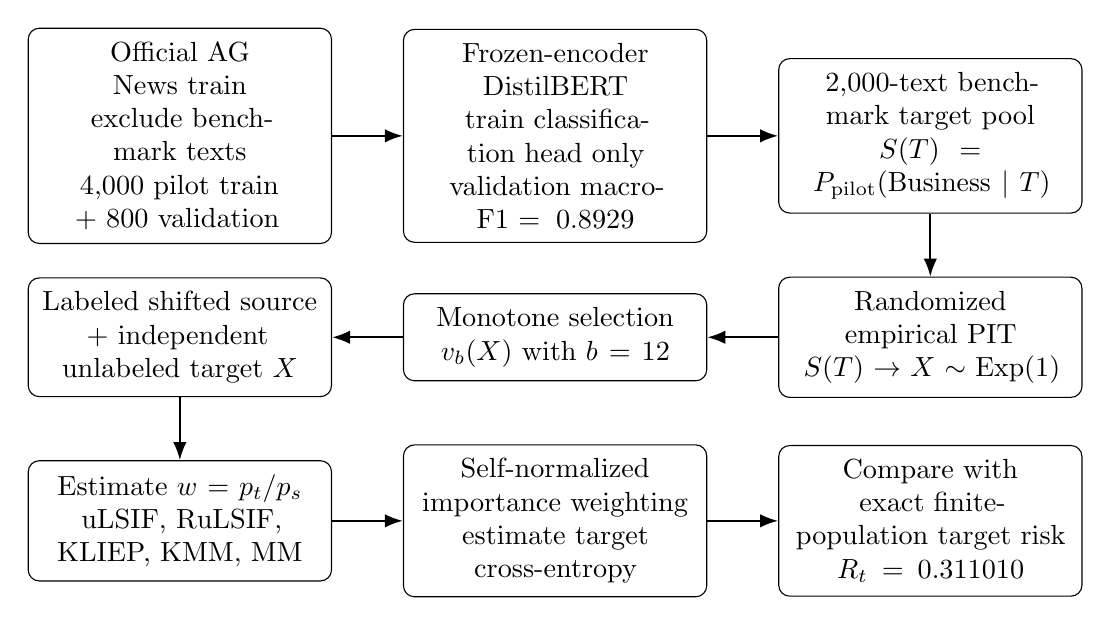
\begin{tikzpicture}[node distance=0.8cm and 0.9cm]
  \node[flowbox] (pdata) {Official AG News train\\exclude benchmark texts\\4,000 pilot train + 800 validation};
  \node[flowbox, right=of pdata] (pilot) {Frozen-encoder DistilBERT\\train classification head only\\validation macro-F1 $=0.8929$};
  \node[flowbox, right=of pilot] (score) {2,000-text benchmark target pool\\$S(T)=P_{\rm pilot}(\mathrm{Business}\mid T)$};

  \node[flowbox, below=of score] (pit) {Randomized empirical PIT\\$S(T)\rightarrow X\sim\mathrm{Exp}(1)$};
  \node[flowbox, left=of pit] (shift) {Monotone selection\\$v_b(X)$ with $b=12$};
  \node[flowbox, left=of shift] (samples) {Labeled shifted source\\+ independent unlabeled target $X$};

  \node[flowbox, below=of samples] (ratio) {Estimate $w=p_t/p_s$\\uLSIF, RuLSIF, KLIEP, KMM, MM};
  \node[flowbox, right=of ratio] (risk) {Self-normalized importance weighting\\estimate target cross-entropy};
  \node[flowbox, right=of risk] (compare) {Compare with exact finite-population target risk\\$R_t=0.311010$};

  \draw[flowarrow] (pdata) -- (pilot);
  \draw[flowarrow] (pilot) -- (score);
  \draw[flowarrow] (score) -- (pit);
  \draw[flowarrow] (pit) -- (shift);
  \draw[flowarrow] (shift) -- (samples);
  \draw[flowarrow] (samples) -- (ratio);
  \draw[flowarrow] (ratio) -- (risk);
  \draw[flowarrow] (risk) -- (compare);
\end{tikzpicture}%
}
\caption{Project pipeline from independent pilot-model training to semantic-shift construction and target-risk estimation.}
\label{fig:pipeline}
\end{figure}

\subsection{Target-risk and density-ratio estimation}

After constructing the shift, I fixed the same independent pilot classifier as the deployed model. I precomputed its cross-entropy loss on every text in the 2,000-example target population. This gives the exact finite-population reference
\[
R_t=0.311010.
\]
These target labels are used only to define the evaluation benchmark, not to fit the density ratio.

For each replicate, I independently drew 1,958 labeled source observations and 2,000 unlabeled target $X$ values. I estimated the target-to-source ratio using uLSIF \citep{kanamori2009least}, RuLSIF \citep{yamada2011relative}, KLIEP \citep{sugiyama2008direct}, KMM \citep{huang2007correcting}, and my monotone MM estimator. The oracle ratio provided a reference method.

Each estimated ratio was converted into the self-normalized importance-weighted risk
\[
\widehat R_t^{SN}=
\frac{\sum_i \widehat w_i\ell_i}
{\sum_i \widehat w_i}.
\]
I repeated the source/target sampling and estimation procedure 100 times and compared bias, standard deviation, MAE, RMSE, weight accuracy, and numerical failures.

\section{Result}

Naive source evaluation substantially overestimated target risk: its mean estimate was 0.3562 versus the true value 0.3110, with RMSE 0.0479. Density-ratio weighting sharply reduced this error.

\begin{table}[H]
\centering
\caption{Target-risk estimation across 100 repeated experiments.}
\label{tab:risk}
\begin{tabular}{lrrrrr}
\toprule
Method & Valid $B$ & Bias & SD & MAE & RMSE \\
\midrule
Naive source & 100 & 0.0452 & 0.0158 & 0.0452 & 0.0479 \\
Oracle       & 100 & 0.0035 & 0.0159 & 0.0133 & 0.0162 \\
uLSIF        & 100 & 0.0052 & 0.0155 & 0.0132 & 0.0163 \\
RuLSIF       & 100 & 0.0128 & 0.0196 & 0.0183 & 0.0234 \\
KLIEP        & 100 & 0.0330 & 0.0258 & 0.0345 & 0.0418 \\
KMM          & 94  & 0.0031 & 0.0158 & 0.0131 & 0.0160 \\
MM           & 100 & 0.0174 & 0.0141 & 0.0187 & 0.0223 \\
\bottomrule
\end{tabular}
\end{table}

uLSIF reduced RMSE by about 66\% relative to naive evaluation while remaining valid in all 100 replications. KMM achieved comparable RMSE when successful, but produced invalid negative weights in 6 replications; I retained these as failures rather than clipping the weights after observing the results.

\begin{figure}[H]
    \centering
    
\includegraphics[width=0.76\textwidth]{figures/target_risk_estimates_boxplot.png}
    \caption{Estimated target cross-entropy across 100 replications. The horizontal line is the exact target risk.}
    \label{fig:boxplot}
\end{figure}

The monotone MM estimator reduced RMSE by about 53\% relative to naive evaluation and was valid in every replication. Its average correlation with oracle weights was 0.973, the highest among the estimated methods. However, its weight variation was smaller than the oracle variation ($CV^2=0.048$ versus 0.097), indicating that MM recovered the weight ordering well but produced a conservative adjustment. This led to a higher-bias, lower-variance risk estimator.

\begin{figure}[H]
    \centering
    
\includegraphics[width=0.70\textwidth]{figures/target_risk_rmse.png}
    \caption{RMSE of target-risk estimates.}
    \label{fig:rmse}
\end{figure}

\section{Takeaways and Limitations}

The project shows that distribution shift can materially bias evaluation even when retraining a pretrained Transformer is not necessary. Density-ratio weighting can use labeled source data and unlabeled target covariates to recover target-domain risk much more accurately; in this benchmark, uLSIF provided the strongest combination of accuracy and numerical stability. The monotone MM method was less accurate in RMSE but fully stable and recovered the oracle weight ordering particularly well, illustrating a practical bias--variance tradeoff from shape-constrained estimation.

The benchmark is intentionally semi-synthetic: the articles are real, while the selection mechanism is controlled so the oracle ratio is available. The shift is summarized by a one-dimensional Transformer-derived semantic score rather than a fully multidimensional deployment shift, and the final experiment focuses on model evaluation rather than weighted retraining.

\bibliographystyle{plainnat}
\bibliography{references}

\end{document}
